\documentclass[11pt]{beamer}

\usepackage[utf8]{inputenc}
\usepackage{xcolor}
\usepackage{caption}
\usepackage[natbibapa]{apacite}
\usepackage{bbm}
\bibliographystyle{apacite}
\renewcommand{\bibsection}{\subsubsection*{\bibname}}
\renewcommand*{\bibfont}{\scriptsize}

\usepackage{pgfplots}
\usepackage{tikz}
\usepackage{subcaption}

\pgfplotsset{compat=1.16}


\usetheme{Ilmenau}
\usecolortheme{lily}
\newcommand{\light}[2][35]{\color{fg!#1}#2}

\DeclareMathOperator*{\argmin}{arg\,min}

% Nicer looking Itemize and enumerate environments
\newenvironment{wideitemize}{\itemize\addtolength{\itemsep}{14pt}}{\enditemize}
\newenvironment{widenumerate}{\enumerate\addtolength{\itemsep}{14pt}}{\endenumerate}


\defbeamertemplate*{footline}{myminiframes theme}
  {%
    \begin{beamercolorbox}[colsep=1.5pt]{upper separation line foot}
    \end{beamercolorbox}
    \begin{beamercolorbox}[ht=2.5ex,dp=1.125ex,%
      leftskip=.3cm,rightskip=.3cm plus1fil]{author in head/foot}%
      \leavevmode{\usebeamerfont{author in head/foot}\insertshortauthor}%
      \hfill%
      {\usebeamerfont{institute in head/foot}\usebeamercolor[fg]{institute in head/foot}\insertshortinstitute}%
    \end{beamercolorbox}%
    \begin{beamercolorbox}[ht=2.5ex,dp=1.125ex,%
      leftskip=.3cm,rightskip=.3cm plus1fil]{title in head/foot}%
      {\usebeamerfont{title in head/foot}\insertshorttitle\hfill \insertframenumber/\inserttotalframenumber}%<-here
    \end{beamercolorbox}%
    \begin{beamercolorbox}[colsep=1.5pt]{lower separation line foot}
    \end{beamercolorbox}
}





\title{From Value-added to Welfare Added: A Social Planner Approach to Education Policy and Statistics.}
\author{
 Tanner S Eastmond\inst{1} \and Nathan Mather\inst{2} \and Michael Ricks\inst{2} \and Julian Betts\inst{1}} 
\date{\vspace{-8ex}}
\institute[]{\inst{1}Department of Economics, University of California San Diego \and \inst{2}Department of Economics, University of Michigan}
\date{}

\begin{document}




%%%%%%%%%%%%%%%%%%%%%%%%%%%%%%%%%%%%%%%%%%%%%%%%%%%%%%%%
%%%%%%%%%%%%%%%%%%%%%% Tile Page. %%%%%%%%%%%%%%%%%%%%%%
%%%%%%%%%%%%%%%%%%%%%%%%%%%%%%%%%%%%%%%%%%%%%%%%%%%%%%%%

\begin{frame}
    \maketitle
\end{frame}




%%%%%%%%%%%%%%%%%%%%%%%%%%%%%%%%%%%%%%%%%%%%%%%%%%%%%%%%
%%%%%%%%%%%%%%%%%%%%% Introduction %%%%%%%%%%%%%%%%%%%%%
%%%%%%%%%%%%%%%%%%%%%%%%%%%%%%%%%%%%%%%%%%%%%%%%%%%%%%%%

\section{Introduction}

%%%%%%%%%%%%%%%%%%%%%%%%%%%%%%%%%%%%%%%%%%%%%%%%%%%%%%%%
%%%%%%%%%%%%%%%%%%%%%%%%%%%%%%%%%%%%%%%%%%%%%%%%%%%%%%%%

\begin{frame}{Value Added Measures: The Goal}

\begin{itemize}
    \item Goal of Value added measures (VAM) are to rank teachers' ``effectiveness''
        \begin{itemize}
            \item Measure post test achievement controlling for a pretest score
        \end{itemize}
    \item VAM do capture something real
    \begin{itemize}
        \item {\color{gray}{\citep{chetty2014measuring2, pope2017multidimensional}}}
    \end{itemize}
    \item There is heterogeneity in test score effects VAM do not catch
    \begin{itemize}
        \item {\color{gray}{\citep{ehrenberg1995teachers, dee2005teacher, lockwood2009, Delgado2020, macartney2021quantitative, condie2014teacher}}}
    \end{itemize}
\end{itemize}

\end{frame}


%%%%%%%%%%%%%%%%%%%%%%%%%%%%%%%%%%%%%%%%%%%%%%%%%%%%%%%%
%%%%%%%%%%%%%%%%%%%%%%%%%%%%%%%%%%%%%%%%%%%%%%%%%%%%%%%%

\begin{frame}{Value Added Measures: A Policy Disconnect}

\begin{itemize}
    \item Theoretical disconnect between education policy goals and use of VAM 
    \begin{itemize}
        \item Policies explicitly target gains in some subpopulations
        \item VAM are mean-oriented statistics: a teacher's average impact on students' scores
        \item Resulting VAM rankings may carry different \textbf{implicit normative} ``welfare weights''
    \end{itemize}
    
    \item  We propose a set of more flexible heterogeneous VAM 
    \begin{itemize}
        \item Assess teachers' heterogeneous impacts along the achievement distribution
        \item  Weight effects according to an \textbf{explicit normative} policy goal or welfare criterion
    \end{itemize}
\end{itemize}

\end{frame}


%%%%%%%%%%%%%%%%%%%%%%%%%%%%%%%%%%%%%%%%%%%%%%%%%%%%%%%%
%%%%%%%%%%%%%%%%%%%%%%%%%%%%%%%%%%%%%%%%%%%%%%%%%%%%%%%%

\begin{frame}{This Project}

\begin{enumerate}
    \item Build a welfare-relevant framework for VAM (and other educational statistics)
    \item Estimate VA heterogeneity in real student-teacher data
    \item Explore the benefits of utilizing heterogeneous estimates
\end{enumerate}

\end{frame}




%%%%%%%%%%%%%%%%%%%%%%%%%%%%%%%%%%%%%%%%%%%%%%%%%%%%%%%%
%%%%%%%%%%%%%%%%%%% Empirical Framework %%%%%%%%%%%%%%%%%%
%%%%%%%%%%%%%%%%%%%%%%%%%%%%%%%%%%%%%%%%%%%%%%%%%%%%%%%%

\section{Empirical Framework}

%%%%%%%%%%%%%%%%%%%%%%%%%%%%%%%%%%%%%%%%%%%%%%%%%%%%%%%%
%%%%%%%%%%%%%%%%%%%%%%%%%%%%%%%%%%%%%%%%%%%%%%%%%%%%%%%%

\begin{frame}{Our Approach to Standard VA}
    We estimate the following:
    
    \begin{gather}
        y_{it} = \alpha + \beta y_{it-1} + \gamma_{j(i)} + \delta X_{it}' + \varepsilon_{it}
    \end{gather}
    
    Where
    \begin{enumerate}
        \item $y_{it}$ is current test score in English language or math
        \item $\gamma_{j(i)}$ are the estimates for VA for teacher $j(i)$
        \item $X_{it}'$ is a vector of demographic, classroom, and school controls
        %lagged score in other subject, lagged average class and school test scores, gender, race, grade, year, English language status, and special education status.
    \end{enumerate}
    
    \only<2>{In the future we will incorporate shrinkage.}
\end{frame}


%%%%%%%%%%%%%%%%%%%%%%%%%%%%%%%%%%%%%%%%%%%%%%%%%%%%%%%%
%%%%%%%%%%%%%%%%%%%%%%%%%%%%%%%%%%%%%%%%%%%%%%%%%%%%%%%%

\begin{frame}{Modeling Value Added As Social Welfare}

\begin{itemize}
    \item We can think of the following social welfare function
    \begin{itemize}
        \item $\omega(x_i,y_i)$ weights: likely based on \textit{ex ante} expected performance
        % Talk about the concavity here?
        \item $v(x_i,y_i)$ value: think achievement, gains, etc.
    \end{itemize}
    \[
    W  = \sum_i \omega(x_i,y_i) v(x_i,y_i) 
    \] 
    
    \item Traditional VAM take the average gains for students among each teacher
    \begin{itemize}
        \item Let $x_i$ be \textit{ex ante} expected performance, estimated as $\hat{y}_i$, then $\tilde{v}(\cdot) = y_i - \hat{y}_i$
    \end{itemize}
    \[
    \hat{W}_{VA}  = \sum_i \frac{(y_i-\hat{y}_i)}{N_{j(i)}} \hspace{3em}
    \]
    
    \item This implies $\omega(x_i,y_i)=\frac{1}{N_j}$, which is (almost) utilitarian

\end{itemize}


\end{frame}


%%%%%%%%%%%%%%%%%%%%%%%%%%%%%%%%%%%%%%%%%%%%%%%%%%%%%%%%
%%%%%%%%%%%%%%%%%%%%%%%%%%%%%%%%%%%%%%%%%%%%%%%%%%%%%%%%

\begin{frame}{``Welfare Added''}

\begin{itemize}
    \item Let $\hat{v}_j(x_i,y_i)$ estimate a teacher's heterogeneous value added, $\mathbb{E}[v(\cdot)|x_i,j]$
    
    \item Then the estimated ``Welfare Added'' by this teacher is  
    \[
    \hat{W}_j  = \sum_{i\in j} \omega(x_i,y_i) \hat{v}_j(x_i,y_i) 
    \] 
    
    \item Consider the following examples:
    \begin{itemize}
        \item Utilitarian: All students are weighted equally $\omega(x_i,y_i) = 1$
        \item Rawlsian: We care only about students below some cutoff, $c$, $\omega(x_i,y_i) = \mathds{1}(x_i\leq c)$
        \item Pareto: We care about the lower achieving students more $ \omega(x_i,y_i)=  \frac{\alpha x_\mathrm{m}^\alpha}{x_i^{\alpha+1}}$ 
    \end{itemize}
    
    %\item But estimating Welfare Added requires an estimate of $\mathbb{E}[v(\cdot)|x_i,j]$
\end{itemize}


\end{frame}


%%%%%%%%%%%%%%%%%%%%%%%%%%%%%%%%%%%%%%%%%%%%%%%%%%%%%%%%
%%%%%%%%%%%%%%%%%%%%%%%%%%%%%%%%%%%%%%%%%%%%%%%%%%%%%%%%

\begin{frame}{Estimating Effect Heterogeneity}

\begin{itemize}
    \item Intuitively, imagine a pointwise approach for estimating $\hat{v}_j(x_i,y_i)$
    
    \item Binning students by \textit{ex ante} expected score and estimating VA has two problems
    \begin{enumerate}
        \item We don't have infinite data, so bins would be too small
        \item We don't actually know the \textit{ex ante} expected score
    \end{enumerate}

    \item $\hat{y}_{it} = \hat{\beta} X_{it}$ consistently predicts expected score, but with error

\end{itemize}

\end{frame}


%%%%%%%%%%%%%%%%%%%%%%%%%%%%%%%%%%%%%%%%%%%%%%%%%%%%%%%%
%%%%%%%%%%%%%%%%%%%%%%%%%%%%%%%%%%%%%%%%%%%%%%%%%%%%%%%%

\begin{frame}{Estimating Effect Heterogeneity}

    We explore two methods to estimate heterogeneity in VAM across the achievement distribution:
    
    \begin{enumerate}
        \item Standard VA including interacted bins for prior test score
        \item Kernel Regression (future)
    \end{enumerate}
    
\end{frame}


%%%%%%%%%%%%%%%%%%%%%%%%%%%%%%%%%%%%%%%%%%%%%%%%%%%%%%%%
%%%%%%%%%%%%%%%%%%%%%%%%%%%%%%%%%%%%%%%%%%%%%%%%%%%%%%%%

% \begin{frame}{Empirical Simulations}

%     \only<1>{
%         We examine the performance of these estimators compared to traditional value added estimates in a series of simulations.
%     }

%     \only<2>{
%         Example:
        
%         \begin{itemize}
%             \item Students have Normally distributed testing ability
%             \item Students are randomly assigned to teachers
%             \item Our welfare weight in these simulations put 4 times more weight on students below the median of prior achievement.
%         \end{itemize}
%     }

%     \includegraphics<3>[width=\textwidth]{slides/Figures/teacher_example_just_truth_1.png}
    
%     \includegraphics<4>[width=\textwidth]{slides/Figures/standard_cent_run_just_stand_3.png}
    
%     \includegraphics<5>[width=\textwidth]{slides/Figures/standard_cent_run_3.png}

% \end{frame}




%%%%%%%%%%%%%%%%%%%%%%%%%%%%%%%%%%%%%%%%%%%%%%%%%%%%%%%%
%%%%%%%%%%%%%%%%%%%%%%%%% Data %%%%%%%%%%%%%%%%%%%%%%%%%
%%%%%%%%%%%%%%%%%%%%%%%%%%%%%%%%%%%%%%%%%%%%%%%%%%%%%%%%

\section{Data}

%%%%%%%%%%%%%%%%%%%%%%%%%%%%%%%%%%%%%%%%%%%%%%%%%%%%%%%%
%%%%%%%%%%%%%%%%%%%%%%%%%%%%%%%%%%%%%%%%%%%%%%%%%%%%%%%%

\begin{frame}{Data}

    \begin{itemize}
        \item We use data from San Diego Unified School District (SDUSD) for the school years 2002-2003 through 2012-2013
        \item For now, we require that a student has test scores for consecutive years and that a teacher teaches at least 50 such students
        \item This leaves 138,285 unique students and 2,165 unique teachers
    \end{itemize}

\end{frame}

%%%%%%%%%%%%%%%%%%%%%%%%%%%%%%%%%%%%%%%%%%%%%%%%%%%%%%%%
%%%%%%%%%%%%%%%%%%%%%%%%%%%%%%%%%%%%%%%%%%%%%%%%%%%%%%%%

% \begin{frame}{Controls and Outcomes}


%     \begin{itemize}
%         \item Our primary controls include lagged rest scores in both math and English language, lagged average class and school test scores in both subjects, gender, race, grade, year, English language status, and special education status.
%         \item In the SDUSD data our primary outcome is standardized test scores in math and English language.
%         \item We also have high school graduation from the SDUSD data and college information from the National Student Clearinghouse data
%     \end{itemize}

% \end{frame}




%%%%%%%%%%%%%%%%%%%%%%%%%%%%%%%%%%%%%%%%%%%%%%%%%%%%%%%%
%%%%%%%%%%%%%%%%%%%%%%%% Results %%%%%%%%%%%%%%%%%%%%%%%
%%%%%%%%%%%%%%%%%%%%%%%%%%%%%%%%%%%%%%%%%%%%%%%%%%%%%%%%

\section{Results}

%%%%%%%%%%%%%%%%%%%%%%%%%%%%%%%%%%%%%%%%%%%%%%%%%%%%%%%%
%%%%%%%%%%%%%%%%%%%%%%%%%%%%%%%%%%%%%%%%%%%%%%%%%%%%%%%%

\begin{frame}{Within Teacher Variation in Value Added}

    \centering
    \only<1>{
        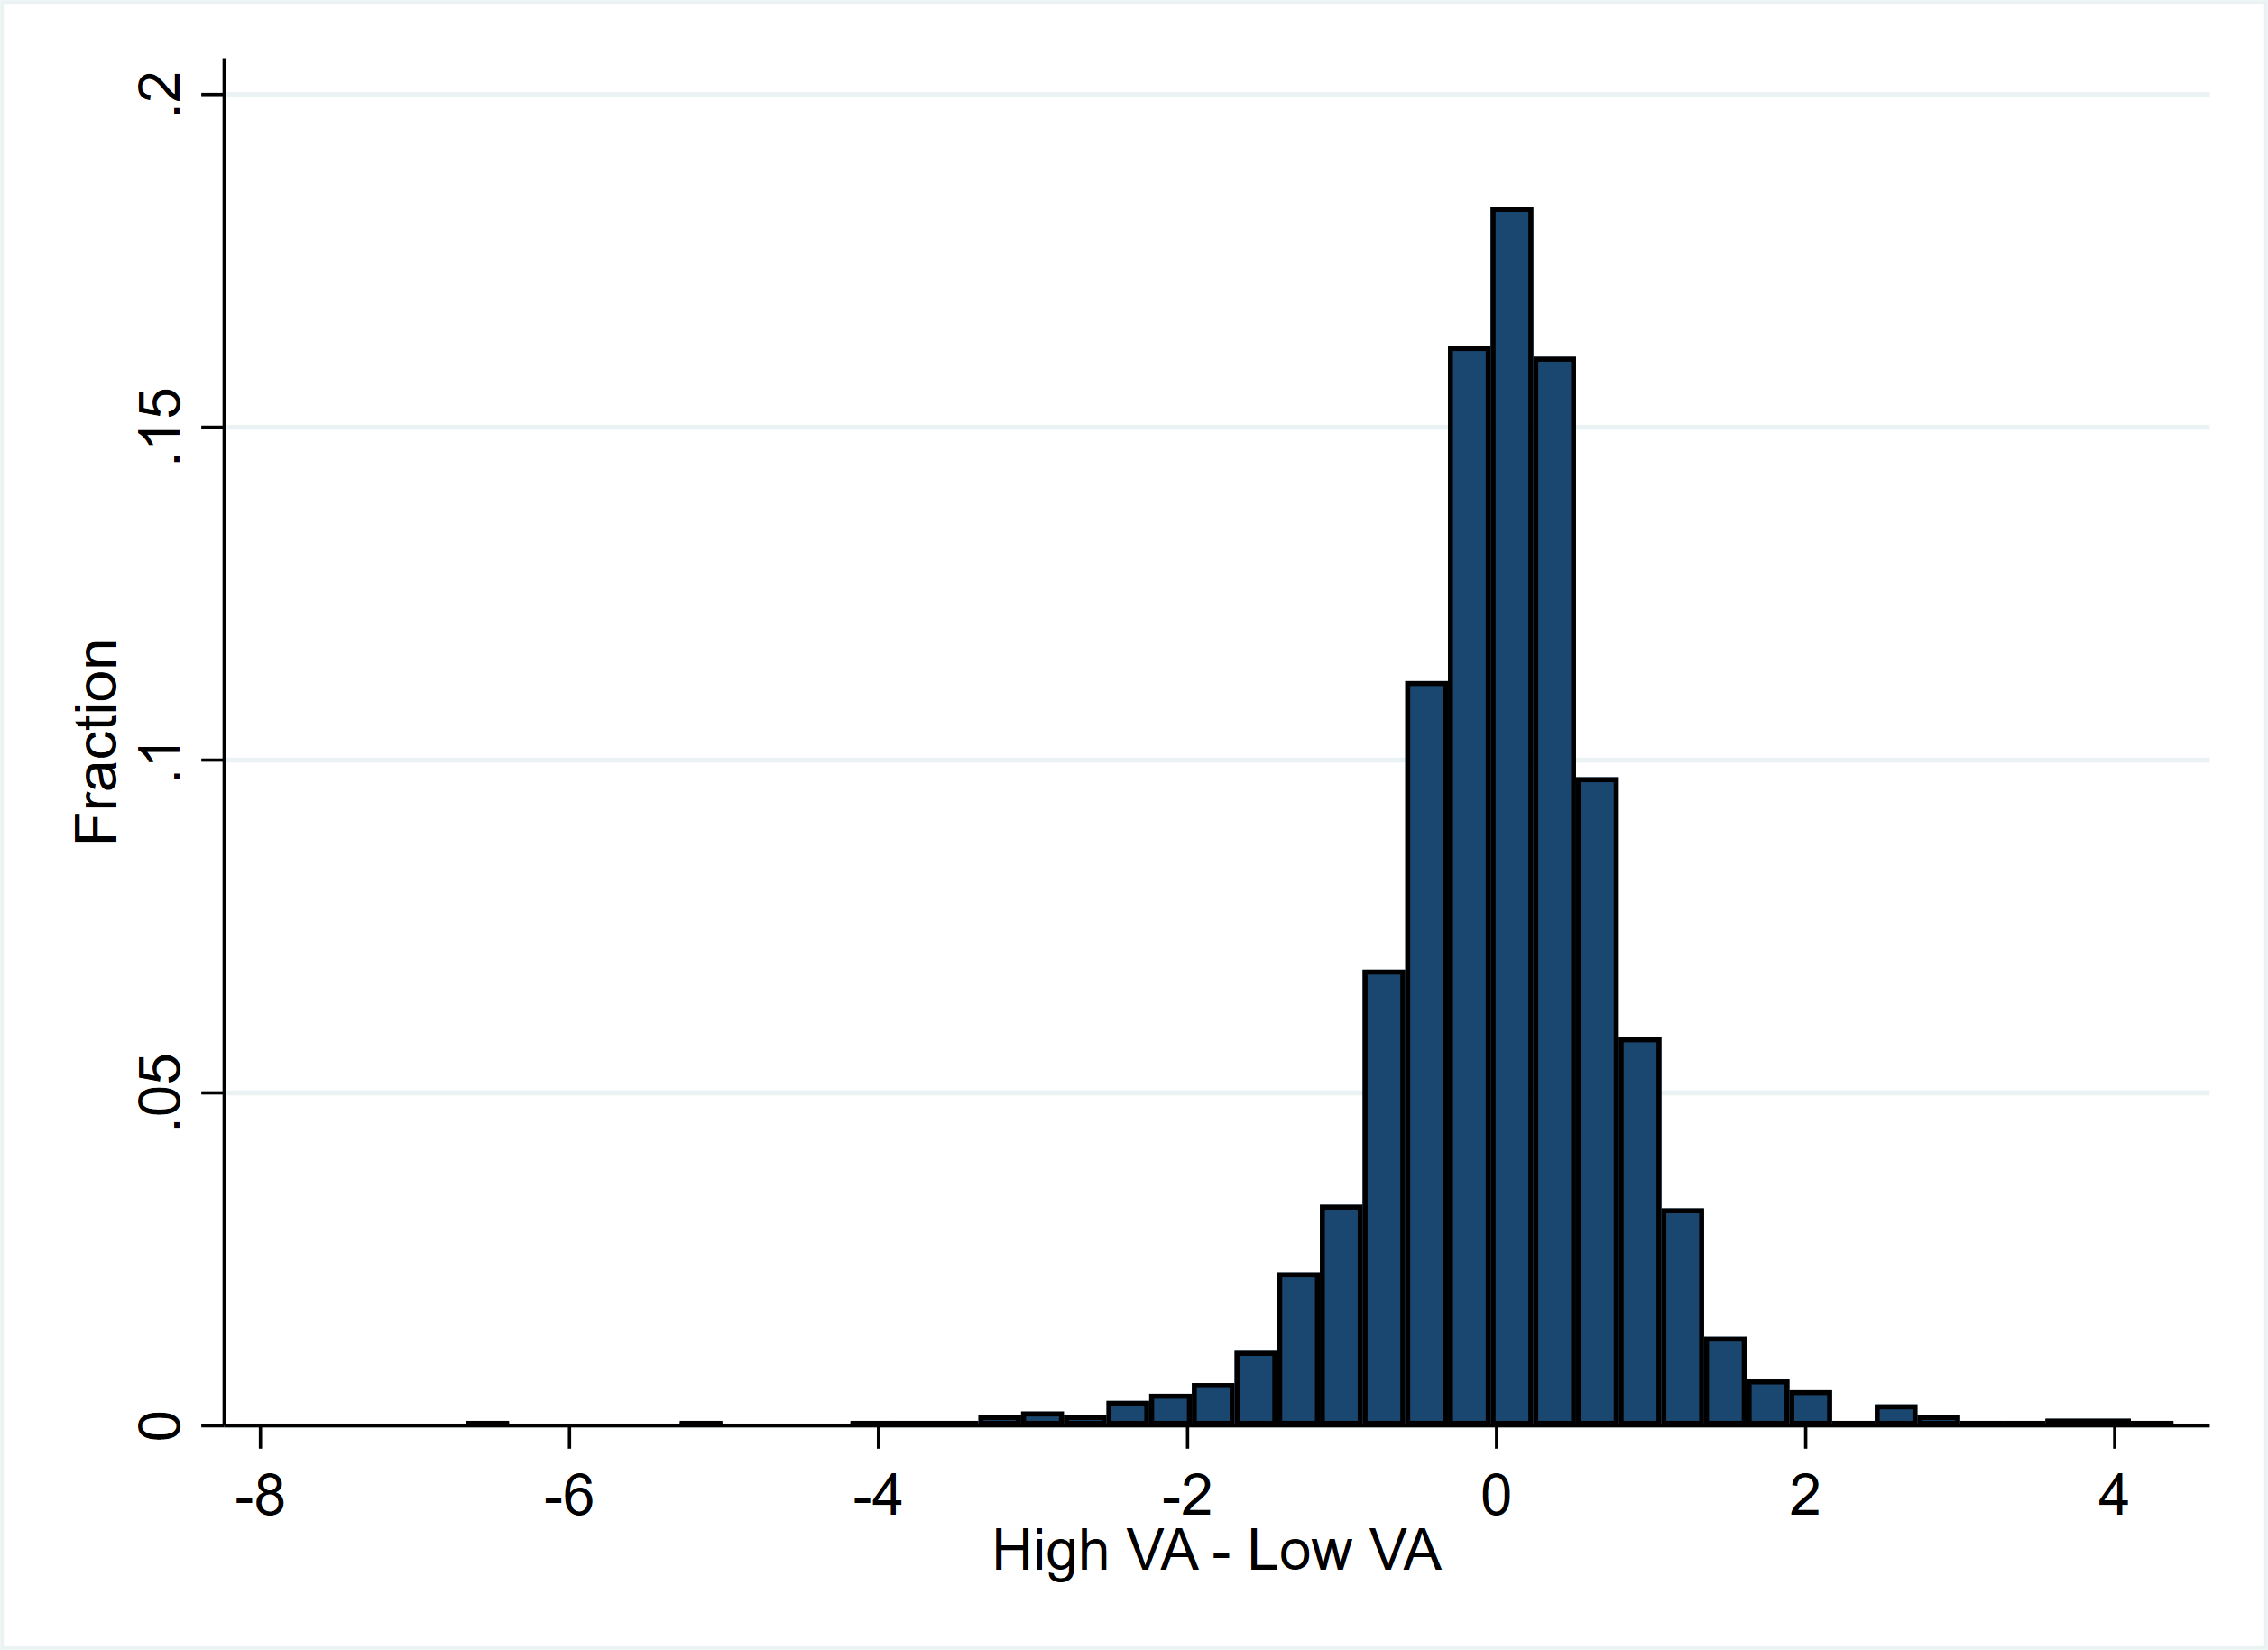
\includegraphics[width=.8\textwidth]{figures/ELA_High_Minus_Low_Hist.png}
    }
    
    \only<2>{
        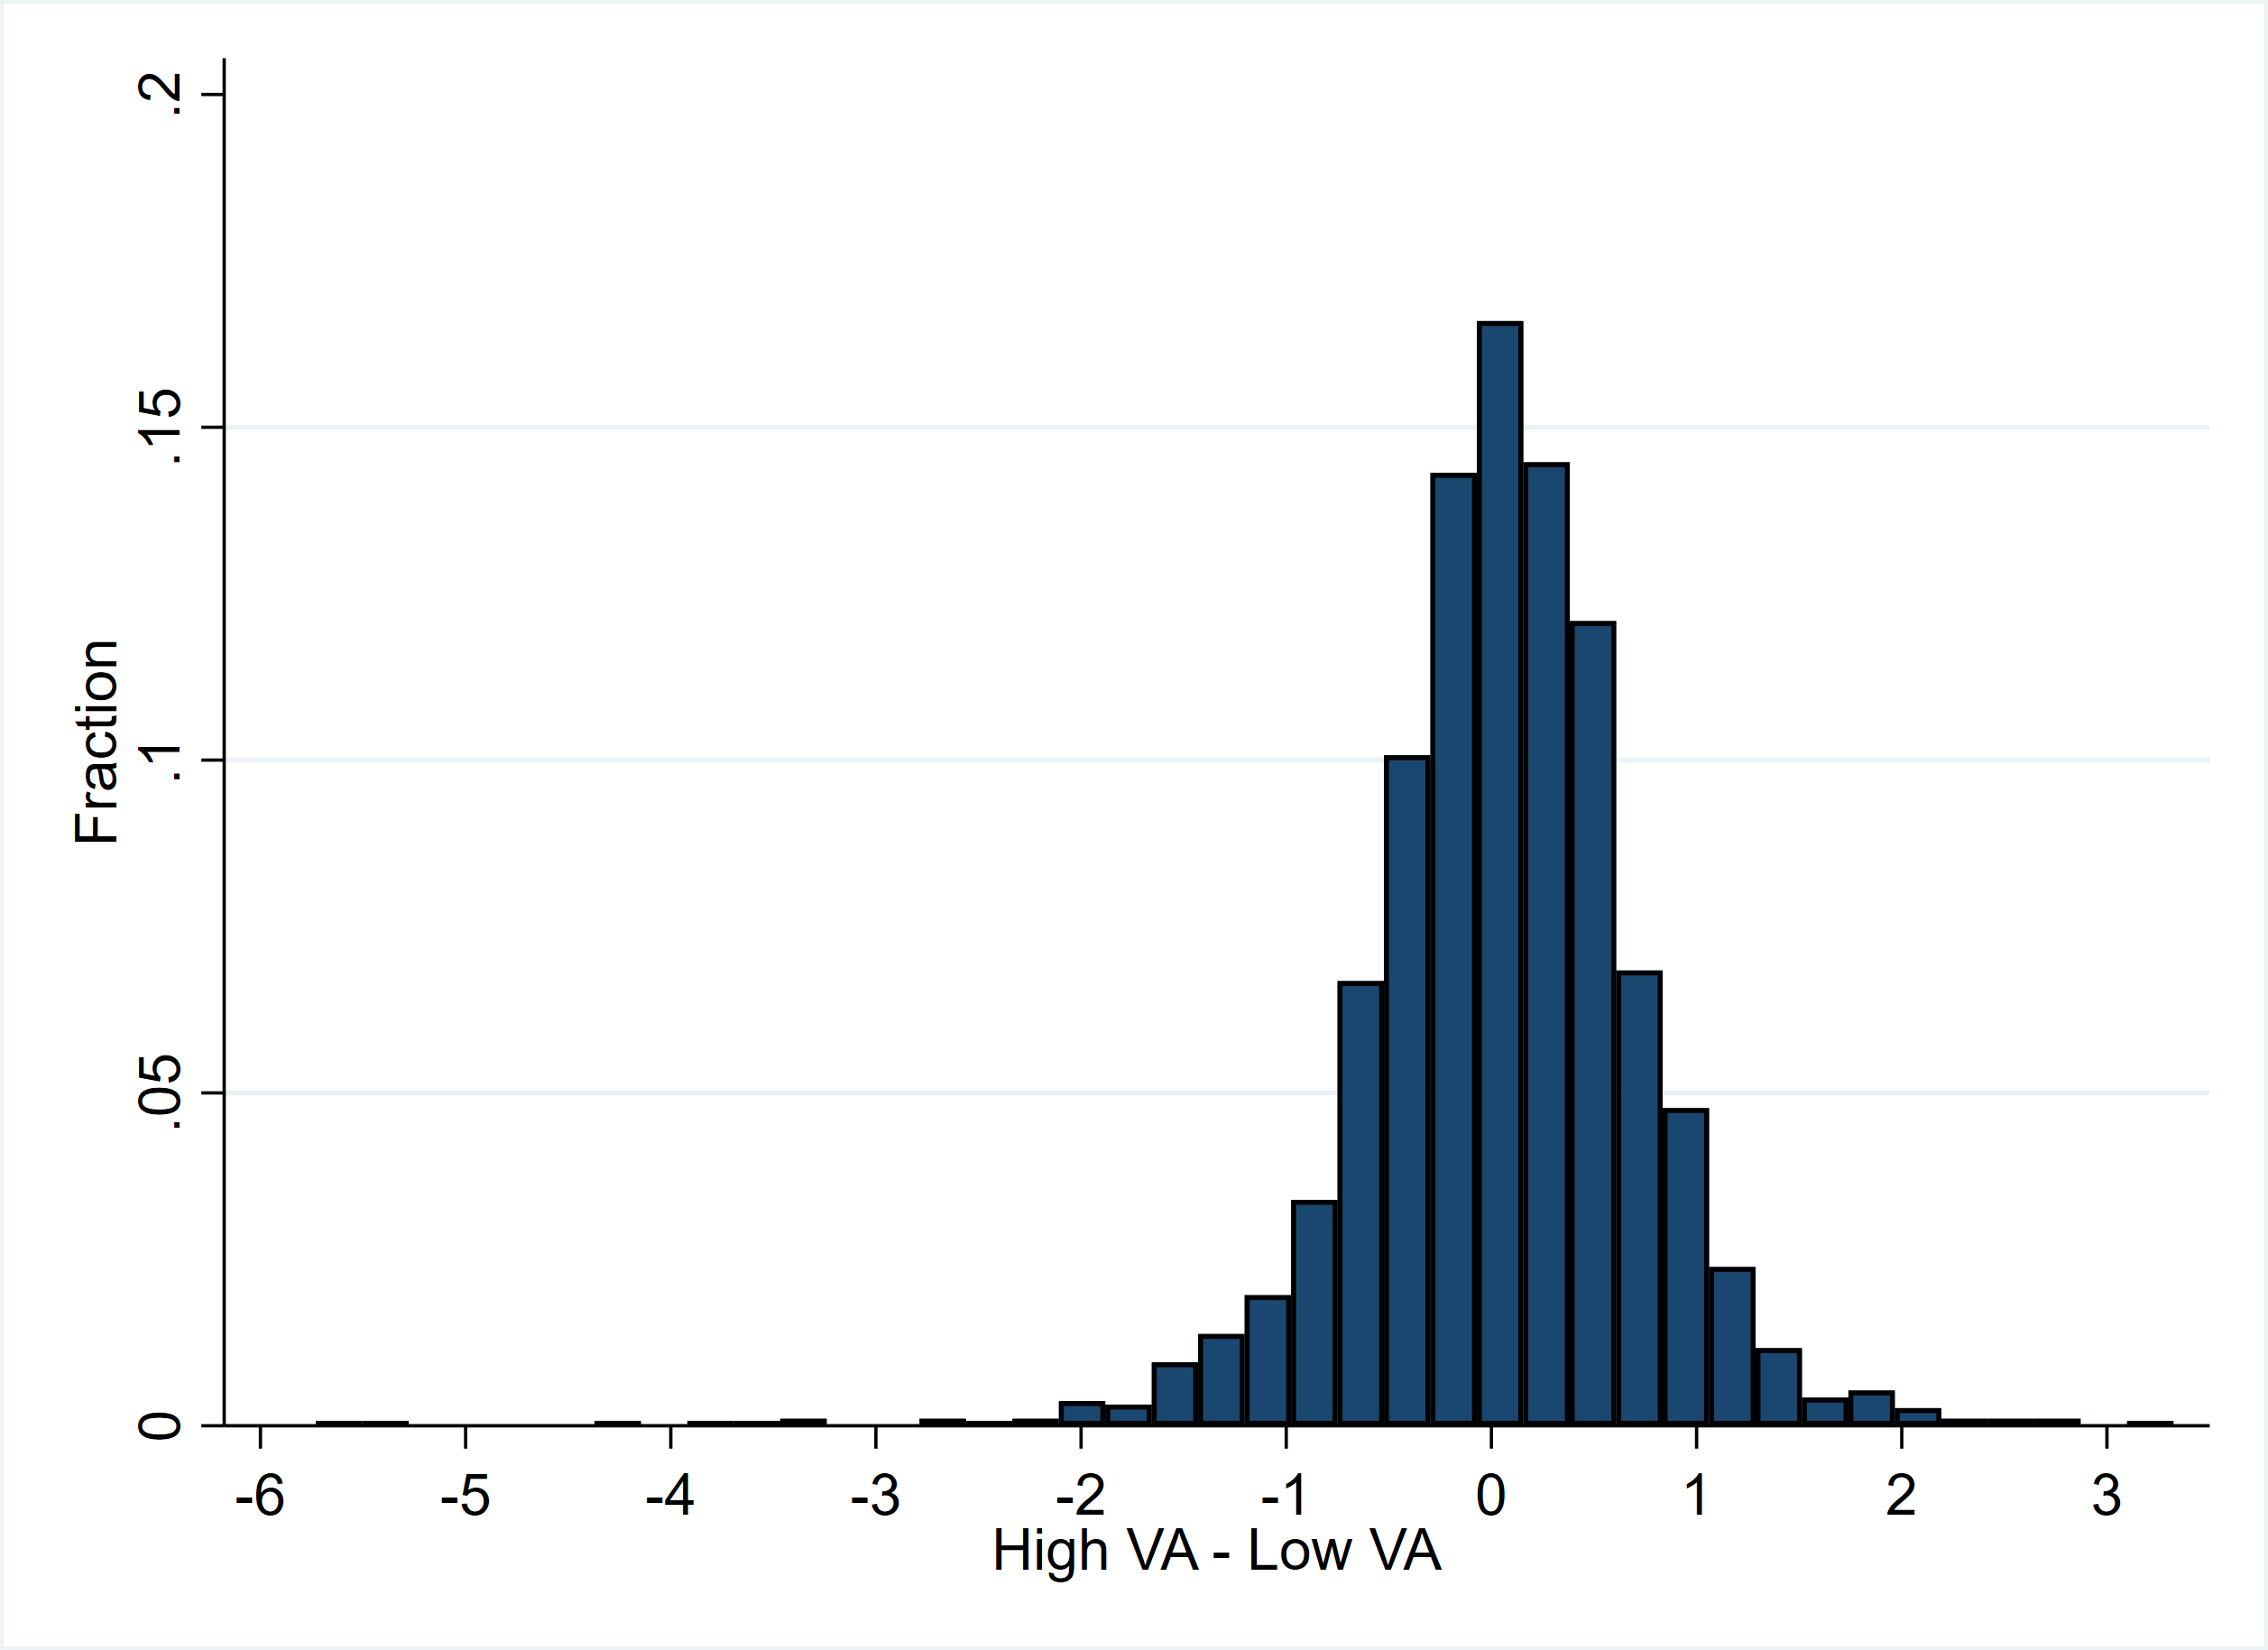
\includegraphics[width=.8\textwidth]{figures/Math_High_Minus_Low_Hist.png}
    }

\end{frame}

%%%%%%%%%%%%%%%%%%%%%%%%%%%%%%%%%%%%%%%%%%%%%%%%%%%%%%%%
%%%%%%%%%%%%%%%%%%%%%%%%%%%%%%%%%%%%%%%%%%%%%%%%%%%%%%%%

\begin{frame}{Long-Term Outcomes}

    \only<1>{
        Graduate from High School
        \centering
        \resizebox{.8\textwidth}{!}{\input{"tables/Highschool Grad"}}
    }
    
    \only<2>{
        Enroll in a 2 year College
        \centering
        \resizebox{.8\textwidth}{!}{\input{"tables/Postsecond 2yr"}}
    }
    
    \only<3>{
        Enroll in a 4 year College
        \centering
        \resizebox{.8\textwidth}{!}{\input{"tables/Postsecond 4yr"}}
    }
    
    \only<4>{
        Bachelor's Degree w/in 6 years after High School
        \centering
        \resizebox{.8\textwidth}{!}{\input{"tables/Bach Degree"}}
    }


\end{frame}


%%%%%%%%%%%%%%%%%%%%%%%%%%%%%%%%%%%%%%%%%%%%%%%%%%%%%%%%
%%%%%%%%%%%%%%%%%%%%%%%%%%%%%%%%%%%%%%%%%%%%%%%%%%%%%%%%

\begin{frame}{Standard VA}

    \only<1>{
    Standard VA estimates have the intuitive appeal that the weight given to students is `utilitarian' in some sense. However, this may be more complicated that simple intuition would suggest.
    }
    \only<2>{
        \centering
        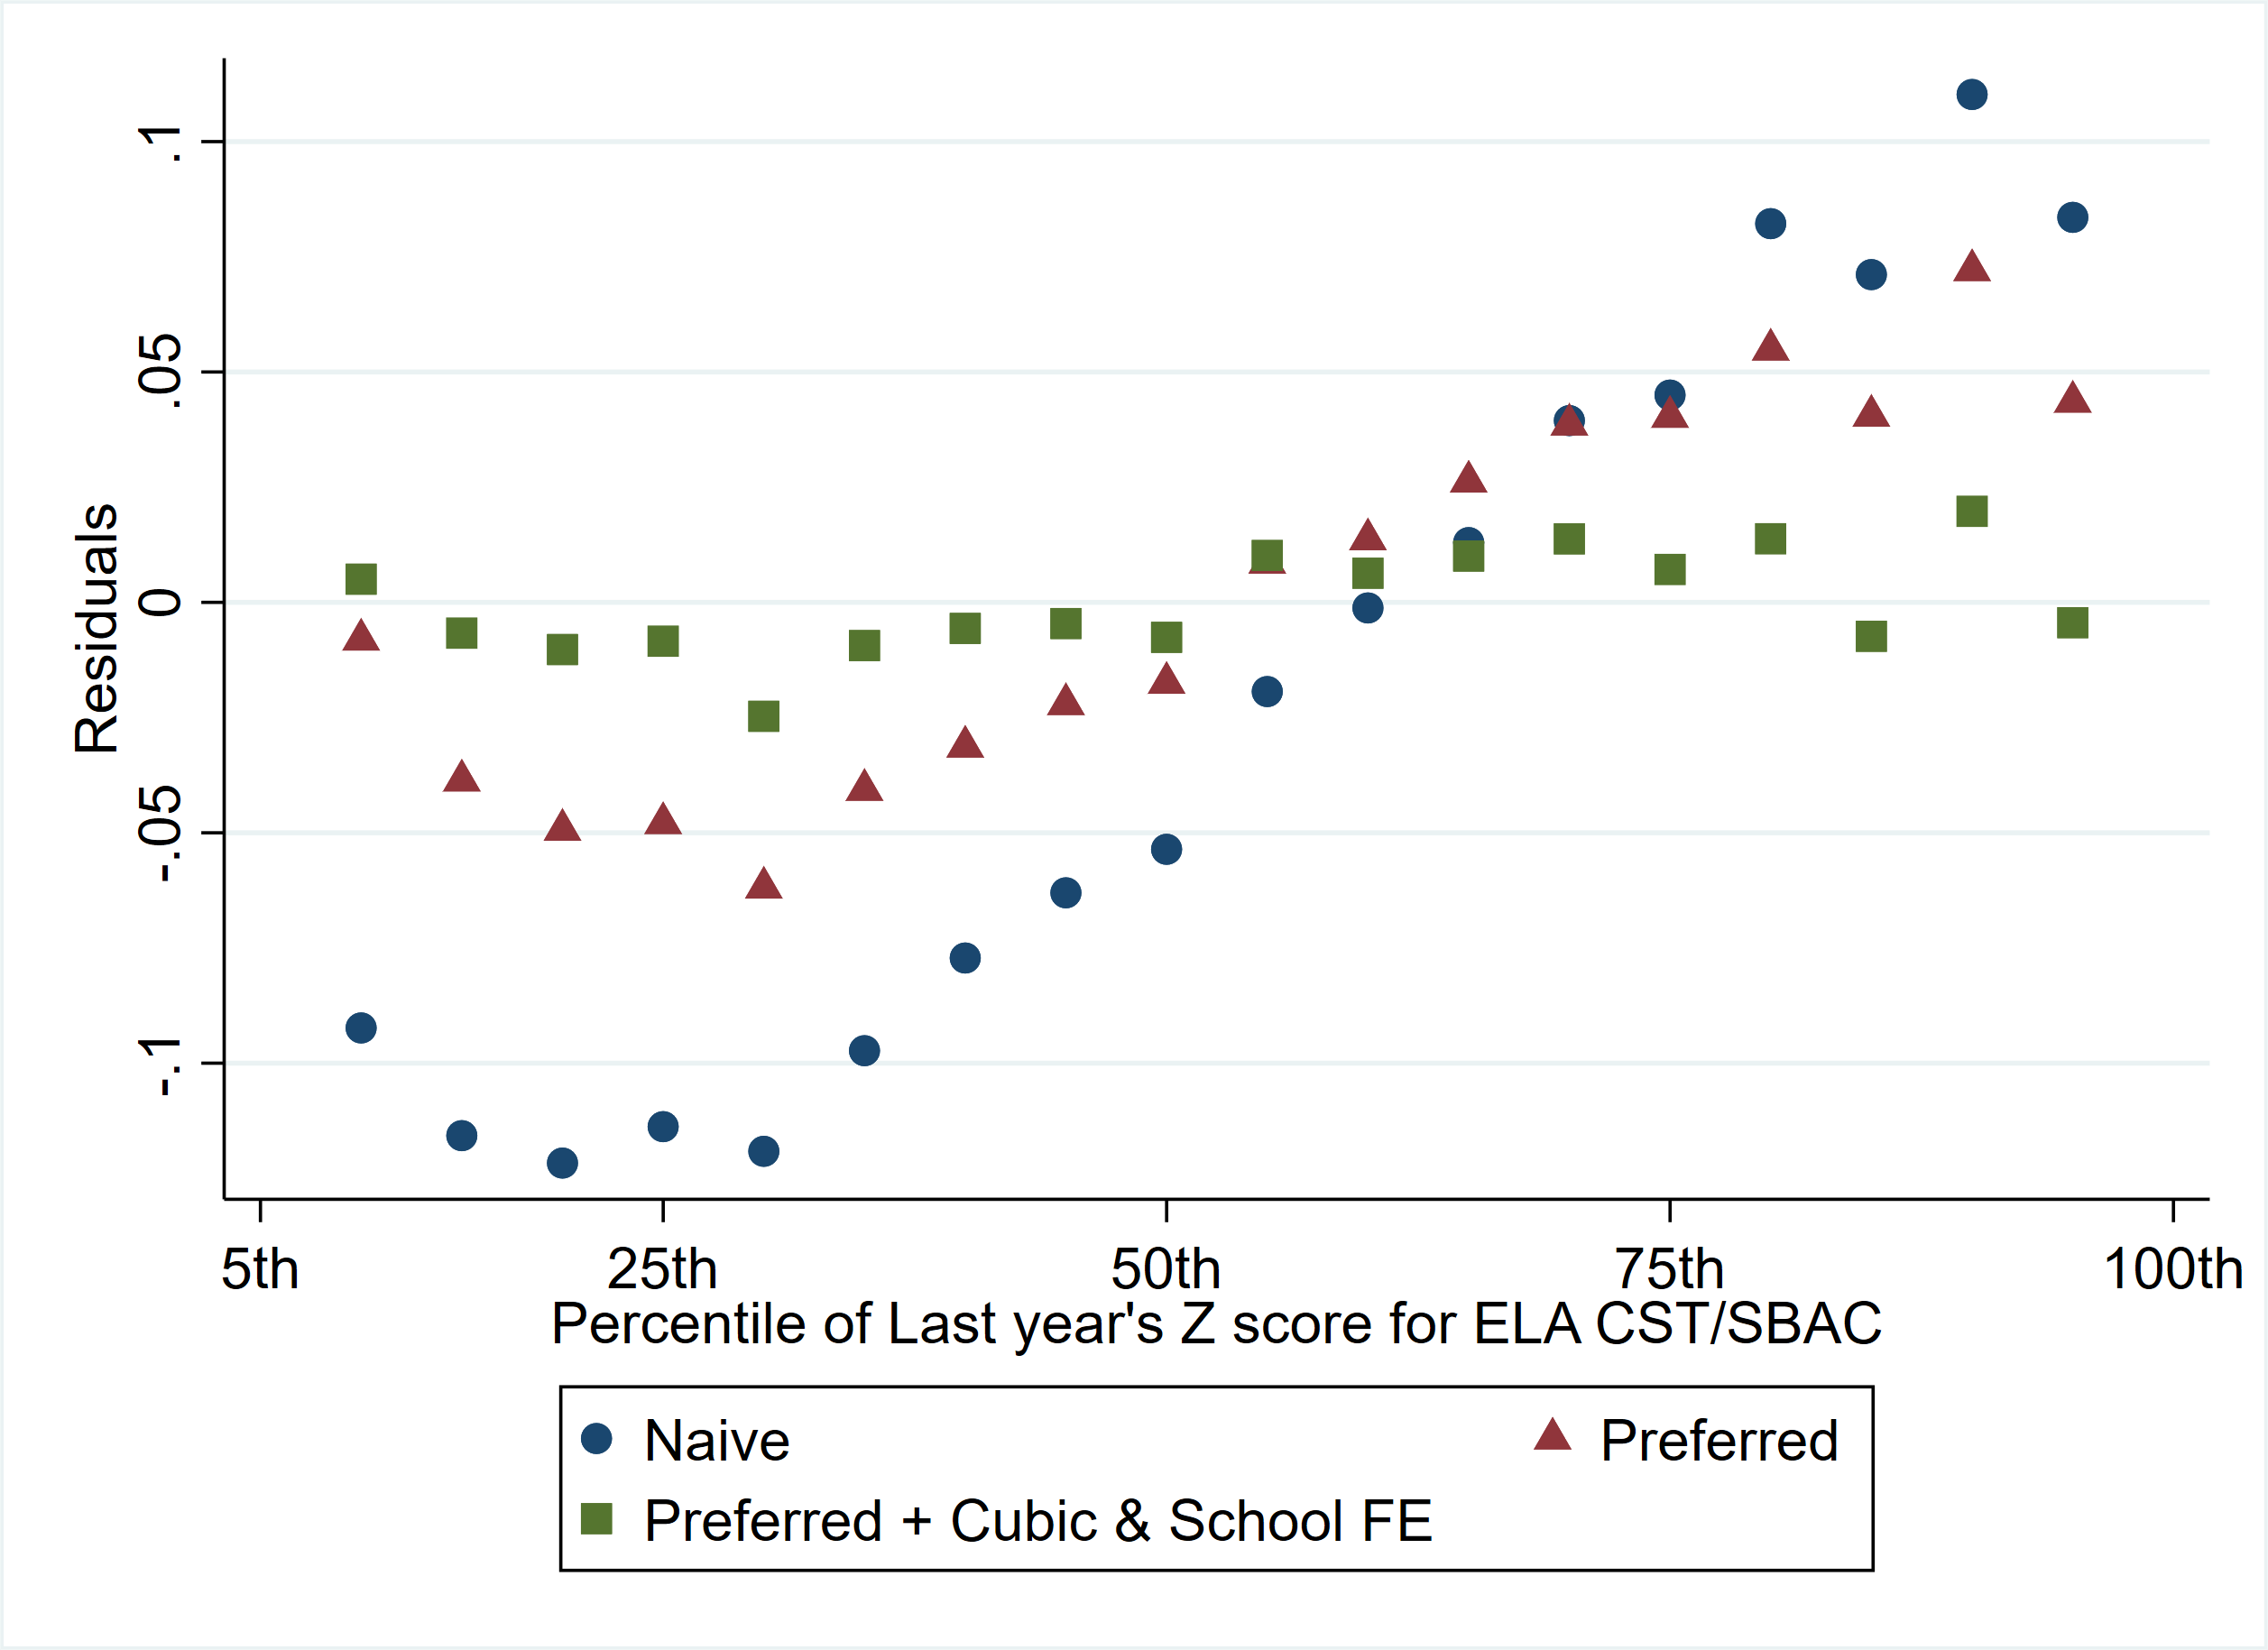
\includegraphics[width=.8\textwidth]{figures/ELA_Resid.png}
    }
    
    \only<3>{
        \centering
        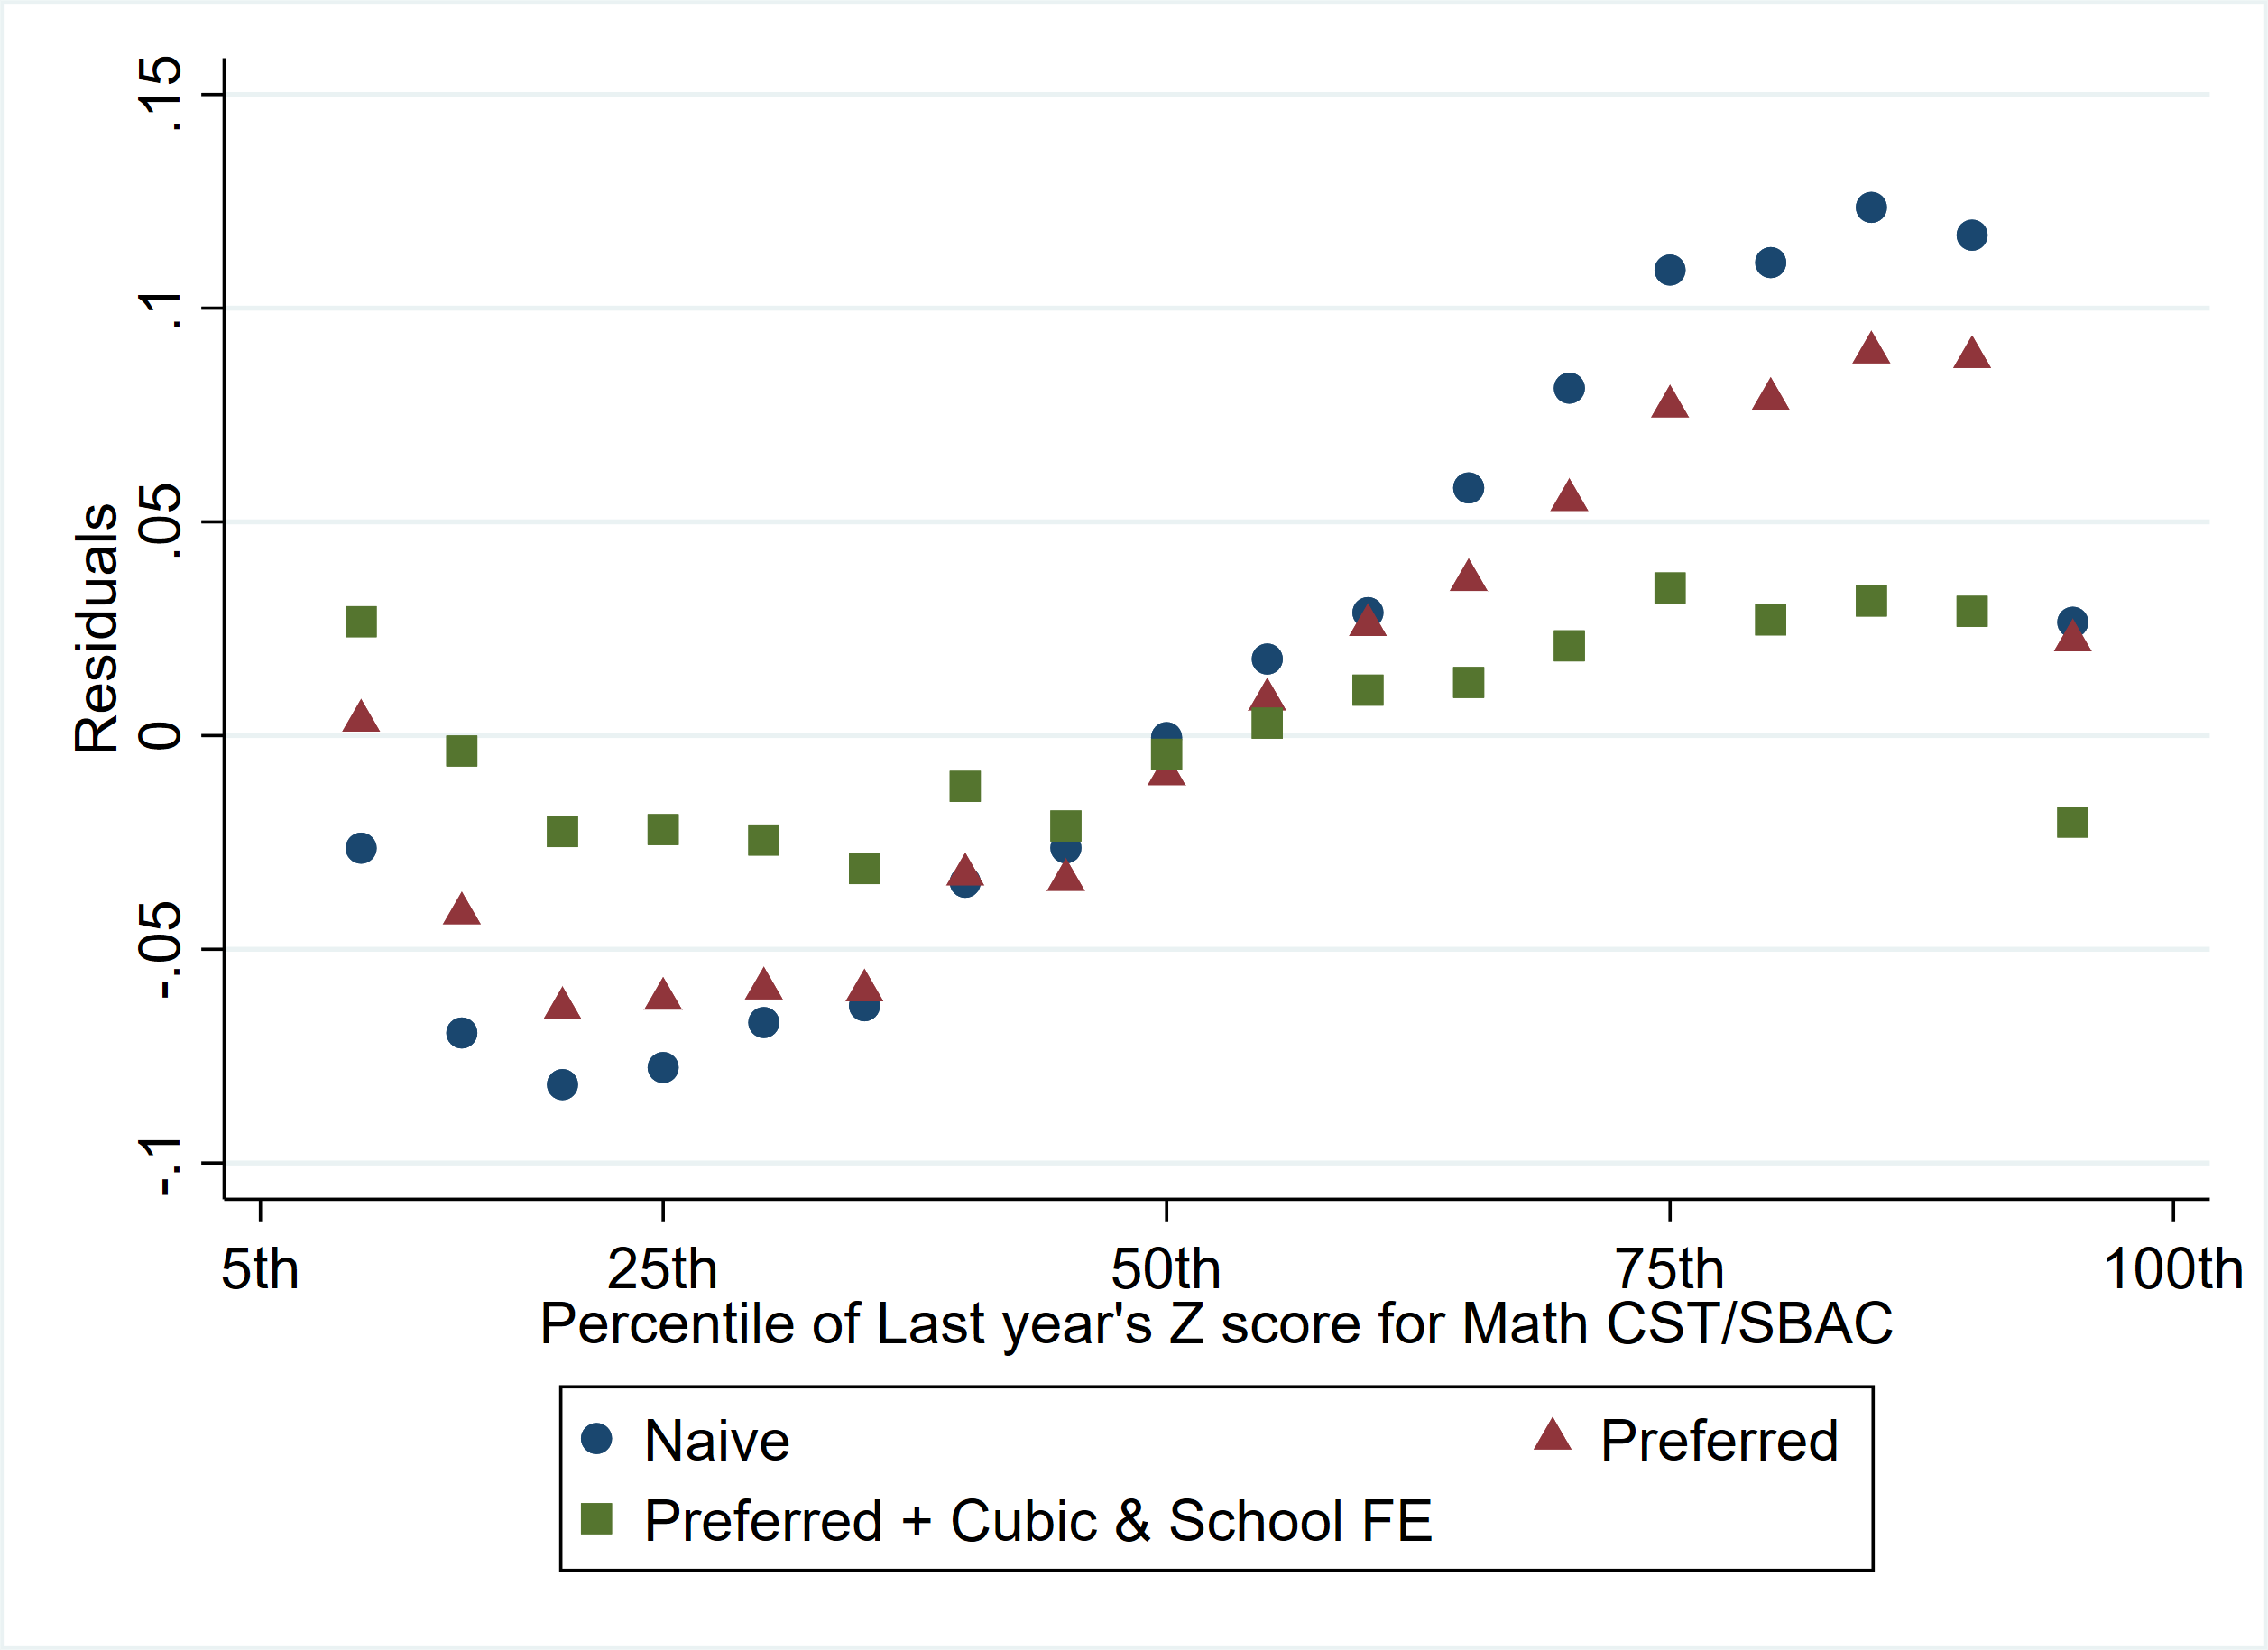
\includegraphics[width=.8\textwidth]{figures/Math_Resid.png}
    }

\end{frame}


%%%%%%%%%%%%%%%%%%%%%%%%%%%%%%%%%%%%%%%%%%%%%%%%%%%%%%%%
%%%%%%%%%%%%%%%%%%%%%%%%%%%%%%%%%%%%%%%%%%%%%%%%%%%%%%%%

\begin{frame}{So what?}

    \only<1>{
    Possible Pareto Gains or re-optimization along PPF.
    
    \centering
    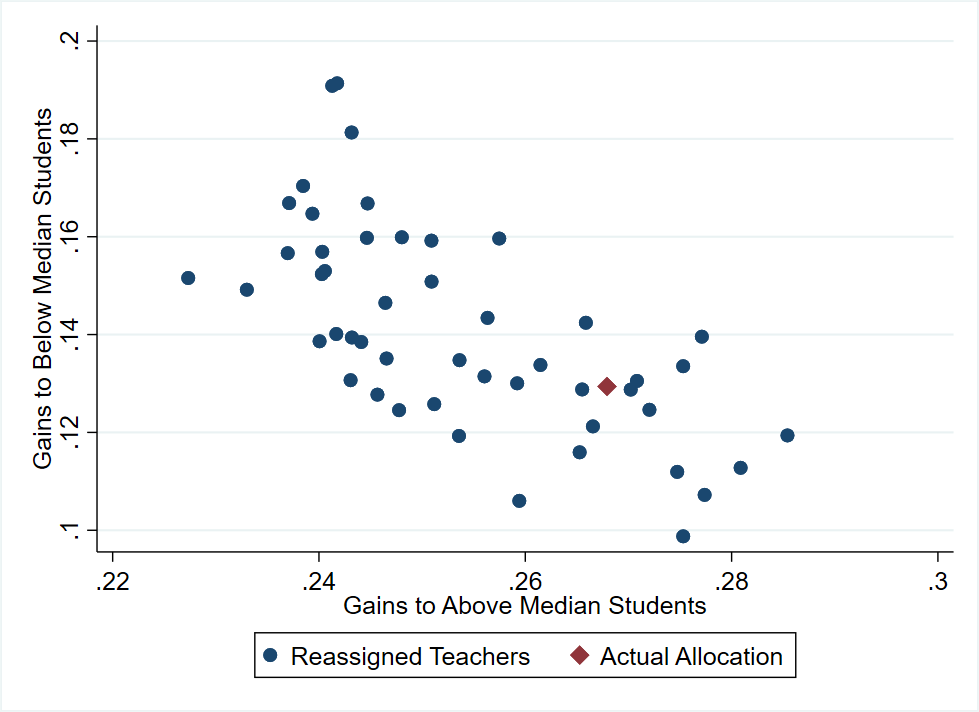
\includegraphics[width=.8\textwidth]{figures/Teacher_PPF.png}
    }
    
    \only<2>{
    Identify teachers pushing forward district goals better for training or incentive purposes.
    }
    
    \only<3>{
    Ensure that incentive schemes do not punish minority students and their teachers.
    }

\end{frame}



%%%%%%%%%%%%%%%%%%%%%%%%%%%%%%%%%%%%%%%%%%%%%%%%%%%%%%%%
%%%%%%%%%%%%%%%%%%%%%%% Conclusion %%%%%%%%%%%%%%%%%%%%%
%%%%%%%%%%%%%%%%%%%%%%%%%%%%%%%%%%%%%%%%%%%%%%%%%%%%%%%%

\section{Conclusion}

%%%%%%%%%%%%%%%%%%%%%%%%%%%%%%%%%%%%%%%%%%%%%%%%%%%%%%%%
%%%%%%%%%%%%%%%%%%%%%%%%%%%%%%%%%%%%%%%%%%%%%%%%%%%%%%%%

\begin{frame}{Conclusion and Next Steps}

    \begin{itemize}
        \item We show evidence that heterogeneity in value added exist for many teachers
        \item This variation appears to be meaningful in terms of long-term outcomes for students
        \item Next steps:
        \begin{itemize}
            \item Can we move away from the two-bin case?
            \item Dig into possible regressivity of Standard VA (effect on minority teachers and students?)
            \item Map out full PPF and `optimal' allocations
        \end{itemize}
    \end{itemize}

\end{frame}



%%%%%%%%%%%%%%%%%%%%%%%%%%%%%%%%%%%%%%%%%%%%%%%%%%%%%%%%
%%%%%%%%%%%%%%%%%%%%%% References %%%%%%%%%%%%%%%%%%%%%%
%%%%%%%%%%%%%%%%%%%%%%%%%%%%%%%%%%%%%%%%%%%%%%%%%%%%%%%%

\section*{}

%%%%%%%%%%%%%%%%%%%%%%%%%%%%%%%%%%%%%%%%%%%%%%%%%%%%%%%%
%%%%%%%%%%%%%%%%%%%%%%%%%%%%%%%%%%%%%%%%%%%%%%%%%%%%%%%%

\begin{frame}[noframenumbering, shrink=15]
    \frametitle{References}
    \centering
    \bibliography{citations}
\end{frame}




%%%%%%%%%%%%%%%%%%%%%%%%%%%%%%%%%%%%%%%%%%%%%%%%%%%%%%%%
%%%%%%%%%%%%%%%%%%%%%%% Appendix %%%%%%%%%%%%%%%%%%%%%%%
%%%%%%%%%%%%%%%%%%%%%%%%%%%%%%%%%%%%%%%%%%%%%%%%%%%%%%%%



\end{document}
